\documentclass{article}

\usepackage{booktabs}
\usepackage{tabularx}
\usepackage{hyperref}
\usepackage{comment}
\usepackage{enumerate}
\usepackage{adjustbox}
\usepackage{booktabs}
\usepackage{multirow}
\usepackage{makecell}
\usepackage{geometry}
\usepackage{graphicx}
\usepackage[shortlabels]{enumitem}
\usepackage{float}
\usepackage{array}
\usepackage{pdflscape}
\usepackage{tabularx,ragged2e,booktabs,caption}
\usepackage{longtable}
\usepackage{ulem}
\usepackage{ltablex}

\hypersetup{
    colorlinks=true,       % false: boxed links; true: colored links
    linkcolor=red,          % color of internal links (change box color with linkbordercolor)
    citecolor=green,        % color of links to bibliography
    filecolor=magenta,      % color of file links
    urlcolor=cyan           % color of external links
}

\title{Hazard Analysis\\\progname}

\author{\authname}

\date{}

%% Comments

\usepackage{color}

\newif\ifcomments\commentstrue %displays comments
%\newif\ifcomments\commentsfalse %so that comments do not display

\ifcomments
\newcommand{\authornote}[3]{\textcolor{#1}{[#3 ---#2]}}
\newcommand{\todo}[1]{\textcolor{red}{[TODO: #1]}}
\else
\newcommand{\authornote}[3]{}
\newcommand{\todo}[1]{}
\fi

\newcommand{\wss}[1]{\authornote{magenta}{SS}{#1}} 
\newcommand{\plt}[1]{\authornote{cyan}{TPLT}{#1}} %For explanation of the template
\newcommand{\an}[1]{\authornote{cyan}{Author}{#1}}

%% Common Parts

\newcommand{\progname}{SFWRENG 4G06 - Capstone Design Process}
\newcommand{\authname}{\textbf{Team 17, DomainX} \\
\\ Awurama Nyarko
\\ Haniye Hamidizadeh
\\ Fei Xie
\\ Ghena Hatoum             
}
\usepackage{hyperref}
    \hypersetup{colorlinks=true, linkcolor=blue, citecolor=blue, filecolor=blue,
                urlcolor=blue, unicode=false}
    \urlstyle{same}
                                


\begin{document}

\maketitle
\thispagestyle{empty}

\pagenumbering{roman}

\begin{table}[hp]
\caption{Revision History} \label{TblRevisionHistory}
\begin{tabularx}{\textwidth}{llX}
\toprule
\textbf{Date} & \textbf{Developer(s)} & \textbf{Change}\\
\midrule
October 6, 2025  & Ghena Hatoum & Added the components\\
October 6, 2025  & Ghena Hatoum & Added the Components Diagram\\
October 6, 2025 & Fei Xie & Added FMEA table\\
... & ... & ...\\
\bottomrule
\end{tabularx}
\end{table}

~\newpage

\tableofcontents

~\newpage


\wss{You are free to modify this template.}

\section{Introduction}

\wss{You can include your definition of what a hazard is here.}

\section{Scope and Purpose of Hazard Analysis}

\wss{You should say what \textbf{loss} could be incurred because of the
hazards.}

\section{System Boundaries and Components}

The following explain the System Components:
\begin{itemize}
    \item Admin UI: Handles invitation, domain creation, and user management views.
    \item Researcher UI: Handles data input, updte, and visualization controls.
    \item User Managment: Handles logic for invite/signup, login, roles, and password reset.
    \item Domain Data Service: Handles read and write operations for Domains, Libraries, and Metrics.
    \item AHP Ranking: Handles the Analytical Hierarchy Process (AHP) calculation.
    \item Visualization: Handles graph generation.
    \item Export: Handles data downloads (JSON/Excel)
    \item Security: Handles Access Control, validation, encrypt password, and manages audit trails.
    \item Persistence: Handles storage and retrieval for all data entities.
    \item System DB: The underlying data store.
\end{itemize}

\begin{figure}[H]
    \centering
    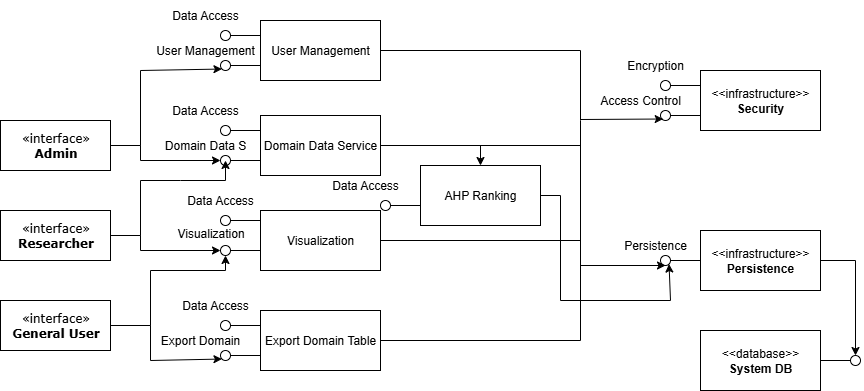
\includegraphics[scale=0.5] {component.png}
\end{figure}

\section{Critical Assumptions}

\wss{These assumptions that are made about the software or system.  You should
minimize the number of assumptions that remove potential hazards.  For instance,
you could assume a part will never fail, but it is generally better to include
this potential failure mode.}

\section{Failure Mode and Effect Analysis}
The following contain our Failure Mode and Effect Analysis table is a breakdown of the hazards that could occur within the system, along with recommanded actions to mitigate them.
\newgeometry{margin=0.5in}
\begin{landscape}
  \begin{longtable}{|p{3cm}|p{3cm}|p{4cm}|p{4cm}|p{3cm}|p{2cm}|p{3cm}|}
  \caption{Failure Mode and Effect Analysis} \label{FMEA}\\
  \hline
   Component & Failure Modes & Effects of Failure & Causes of Failure & Recommended Action & SR & Ref.  \\ 
  \hline
  \endfirsthead
  \multicolumn{7}{r}{Table \thetable\ Continued from previous page}\\ 
  \hline
   Design Function & Failure Modes & Effects of Failure & Causes of Failure & Recommended Action & SR & Ref.  \\ 
  \hline
  \endhead
  \multicolumn{7}{r}{{Continued on next page}}\\
  \endfoot
  \multicolumn{7}{r}{{Concluded}}\\
  \endlastfoot
  \multirow{7}{*}{User account} & 
  \begin{enumerate}[leftmargin=*]
    \item User can't login/signup.
    \item Cannot set correct role for user.
    \item User account information is leaked.
  \end{enumerate} & 
  \begin{enumerate}[leftmargin=*]
    \item User cannot access their work.
    \item Refer to H1-1.
    \item User credentials are exposed, exposing them to cyber attack or data scrapers.
  \end{enumerate} &
  \begin{enumerate}[leftmargin=*]
    \item
    \begin{enumerate}
        \item[a)] Integration with database failure.
        \item[b)] User entered incorrect credentials.
    \end{enumerate}
    \item Refer to H1-1.a.
    \item Weak access controls, lack of encryption, or insecure credentials.
  \end{enumerate} &
  \begin{enumerate}[leftmargin=*]
    \item 
    \begin{enumerate}
        \item[a)] Implement automated daily system integration testing.
        \item[b)] Provide user feedback during user actions.
    \end{enumerate}
    \item Refer to H1-1.a, H1-1.b.
    \item Implement Multi-factor authentication and follow industry best practices for security.
  \end{enumerate} &
  \begin{enumerate}[leftmargin=*]
    \item TODO
    \item TODO
    \item TODO
  \end{enumerate} &
  \begin{enumerate}[leftmargin=*]
    \item H1-1
    \item H1-2
    \item H1-3
  \end{enumerate} \\
  \hline
    Domain Creation & 
  \begin{enumerate}[leftmargin=*]
      \item Cannot create new domains
      \item Cannot edit existing domain
  \end{enumerate} & 
  \begin{enumerate}[leftmargin=*]
    \item
    \begin{enumerate}
        \item[a)] User cannot continue their work on the domain
        \item[b)] User will be delayed when writing their anaylsis
    \end{enumerate}
    \item Refer to H2-1.a, H2-1.b.
  \end{enumerate} &
  \begin{enumerate}[leftmargin=*]
    \item  Refer to H1-1.a
    \begin{enumerate}
        \item[a)] User has incorrect role credentials
    \end{enumerate}
    \item Refer to H1-1.a, H2-1.a.
  \end{enumerate} &
  \begin{enumerate}[leftmargin=*]
       \item Refer to H1-1.a, H1-1.b.
       \item  Refer to H1-1.a, H1-1.b.
  \end{enumerate} &
  \begin{enumerate}[leftmargin=*]
       \item TODO
       \item TODO
  \end{enumerate} &
  \begin{enumerate}[leftmargin=*]
       \item H2-1
       \item H2-2
  \end{enumerate} \\
  \hline
  Adding Data to Domain & 
  \begin{enumerate}[leftmargin=*]
      \item User cannot add new datapoint
      \item User cannot update existing datapoint
      \item Automated process overwriting user data unknowningly
      \item Automated data input failure
  \end{enumerate} & 
  \begin{enumerate}[leftmargin=*]
      \item Refer to H2-1.a, H2-1.b.
      \item Refer to H2-1.a, H2-1.b.
      \item Refer to H2-1.a, H2-1.b 
      \begin{enumerate}
        \item[a)] Loss of user trust towards the tool
    \end{enumerate}
      \item Refer to H2-1.a, H2-1.b,
      \begin{enumerate}
        \item[a)] User has to manually input data, reducing usefulness of the tool
    \end{enumerate}
  \end{enumerate} &
  \begin{enumerate}[leftmargin=*]
       \item Refer to H1-1.a
       \begin{enumerate}
            \item[a)] Network issues
            \item[b)] Save conflict occuring when multiple users are trying to edit the same datapoint
        \end{enumerate}
       \item Refer to H1-1.a, H3-1.a, H3-1.b
       \item 
       \begin{enumerate}
            \item[a)] Lack of user training on how automated datapoints work
            \item[b)] Inadequate user feedback user during system processes
        \end{enumerate}
       \item Refer to H3-1.a.
       \begin{enumerate}
            \item[a)] Integration issues with external systems
        \end{enumerate}
  \end{enumerate} &
  \begin{enumerate}[leftmargin=*]
    \item Refer to H1-1.a, H1-1.b.
    \begin{enumerate}
        \item[a)] Explicit visual block on datapoints that other users are editing
    \end{enumerate}
    \item Refer to H1-1.a, H1-1.b, H3-1.a.
    \item Refer to H1-1.a, H1-1.b
    \begin{enumerate}
        \item[a)] Provide explict user controls for manual inputs
        \item[b)] Provide training on key features to user
        \item[c)] Implement confirmation system for automated sections
    \end{enumerate}
    \item Refer to H1-1.a, H1-1.b, H3-1.a.
  \end{enumerate} &
  \begin{enumerate}[leftmargin=*]
    \item TODO
    \item TODO
    \item TODO
    \item TODO

  \end{enumerate} &
  \begin{enumerate}[leftmargin=*]
    \item H3-1
    \item H3-2
    \item H3-3
    \item H3-4
  \end{enumerate} \\
  \hline
 Data Visualization & 
  \begin{enumerate}[leftmargin=*]
      \item Visualization method does not match datapoints
  \end{enumerate} & 
  \begin{enumerate}[leftmargin=*]
      \item Refer to H2-1.b, H3-3.a.
  \end{enumerate} &
  \begin{enumerate}[leftmargin=*]
    \item Refer to H1-1.a
    \begin{enumerate}
        \item[a)] External system used for visualization not properly configured/working
        \item[b)] Another user is editing the datapoints while current user is trying to visualize
    \end{enumerate}
  \end{enumerate} &
  \begin{enumerate}[leftmargin=*]
    \item Refer to H1-1.A
    \begin{enumerate}
        \item[a)] Require user to lock the domain when editing, with visualization functionality being available only on un-locked domains.
    \end{enumerate}
  \end{enumerate} &
  \begin{enumerate}[leftmargin=*]
       \item TODO
  \end{enumerate} &
  \begin{enumerate}[leftmargin=*]
       \item H4-1
  \end{enumerate} \\
  \hline
 Download Data  & 
  \begin{enumerate}[leftmargin=*]
    \item User unable to download the data/visuals of a domain
    \item Downloaded data/visuals of a domain are corrupted and unusable
  \end{enumerate} & 
  \begin{enumerate}[leftmargin=*]
      \item Refer to H2-1.b.
      \item Refer to H2-1.b, H3-3.a.
  \end{enumerate} &
  \begin{enumerate}[leftmargin=*]
    \item Refer to H1-1.a, H2.1.a, H3-1.a, H4-1.a.
    \item Refer to H1-1.a, H3-1.a, H4-1.a.
  \end{enumerate} &
  \begin{enumerate}[leftmargin=*]
       \item Refer tp H1-1.a, H1-1.b.
       \begin{enumerate}
        \item[a)] Provide multiple methods for downloading or sharing
    \end{enumerate}
       \item Refer tp H1-1.a, H1-1.b.
       \begin{enumerate}
        \item[a)] Implement proper error handling in code to catch exceptions
    \end{enumerate}
  \end{enumerate} &
  \begin{enumerate}[leftmargin=*]
       \item TODO
       \item TODO
  \end{enumerate} &
  \begin{enumerate}[leftmargin=*]
       \item H5-1
       \item H5-2
  \end{enumerate} \\
  \hline
  \end{longtable}
\end{landscape}
\restoregeometry


\section{Safety and Security Requirements}

\wss{Newly discovered requirements.  These should also be added to the SRS.  (A
rationale design process how and why to fake it.)}

\section{Roadmap}

\wss{Which safety requirements will be implemented as part of the capstone timeline?
Which requirements will be implemented in the future?}

\newpage{}

\section*{Appendix --- Reflection}

\wss{Not required for CAS 741}

The purpose of reflection questions is to give you a chance to assess your own
learning and that of your group as a whole, and to find ways to improve in the
future. Reflection is an important part of the learning process.  Reflection is
also an essential component of a successful software development process.  

Reflections are most interesting and useful when they're honest, even if the
stories they tell are imperfect. You will be marked based on your depth of
thought and analysis, and not based on the content of the reflections
themselves. Thus, for full marks we encourage you to answer openly and honestly
and to avoid simply writing ``what you think the evaluator wants to hear.''

Please answer the following questions.  Some questions can be answered on the
team level, but where appropriate, each team member should write their own
response:


\begin{enumerate}
    \item What went well while writing this deliverable? 
    \item What pain points did you experience during this deliverable, and how
    did you resolve them?
    \item Which of your listed risks had your team thought of before this
    deliverable, and which did you think of while doing this deliverable? For
    the latter ones (ones you thought of while doing the Hazard Analysis), how
    did they come about?
    \item Other than the risk of physical harm (some projects may not have any
    appreciable risks of this form), list at least 2 other types of risk in
    software products. Why are they important to consider?
\end{enumerate}

\end{document}